\section{Latch D vs Flip-Flop D \label{sec:s4}}

\begin{center}
	\begin{minipage}{12cm}
		\begin{tcolorbox}[title=Actividad 4]
			Repetir el inciso 3 pero indicando codificación \textit{``ONE - HOT''}. ¿Qué códigos \textit{ONE-HOT} fueron utilizados, como los de la tabla normal o la modificada?
		\end{tcolorbox}	
	\end{minipage}
\end{center}

La visualización RTL, del latch D descrito por comportamiento, se muestra en la \autoref{fig:L_D_RTL} y del flip flop D descrito por comportamiento en la \autoref{fig:FF_D_RTL}. Ahora bien, a través del \textit{Chip Planner} se observa que el latch D se implementa en el elemento lógico de la \autoref{fig:L_D_CP} y el flip-flop D en el elemento de la \autoref{fig:FF_D_CP} (Ver en la \autoref{fig:L_D_CP2} y en la \autoref{fig:FF_D_CP2} a los elementos acercados). Aunque pareciera que el latch D y el flip-flop D se efectúan de igual forma en un elemento lógico, se observa en la \autoref{fig:L_D_CP3} que el latch se implementa en la \textit{Look Up Table} de un elemento lógico, mientras que en la \autoref{fig:FF_D_CP3} se ve que el flip-flop se implementa de forma directa en el elemento lógico.

Las simulaciones se visualizan en la \autoref{fig:L_D_Wave} para el latch D y en la \autoref{fig:FF_D_Wave} para el flip-flop D. Se visualiza un correcto funcionamiento de ambos módulos, ya que el latch varía a la salida cuando en CLK hay un cambio al nivel lógico alto, mientras que el flip-flop lo hace con un flaco de subida en CLK.

\begin{figure}[ht]
	\centering
	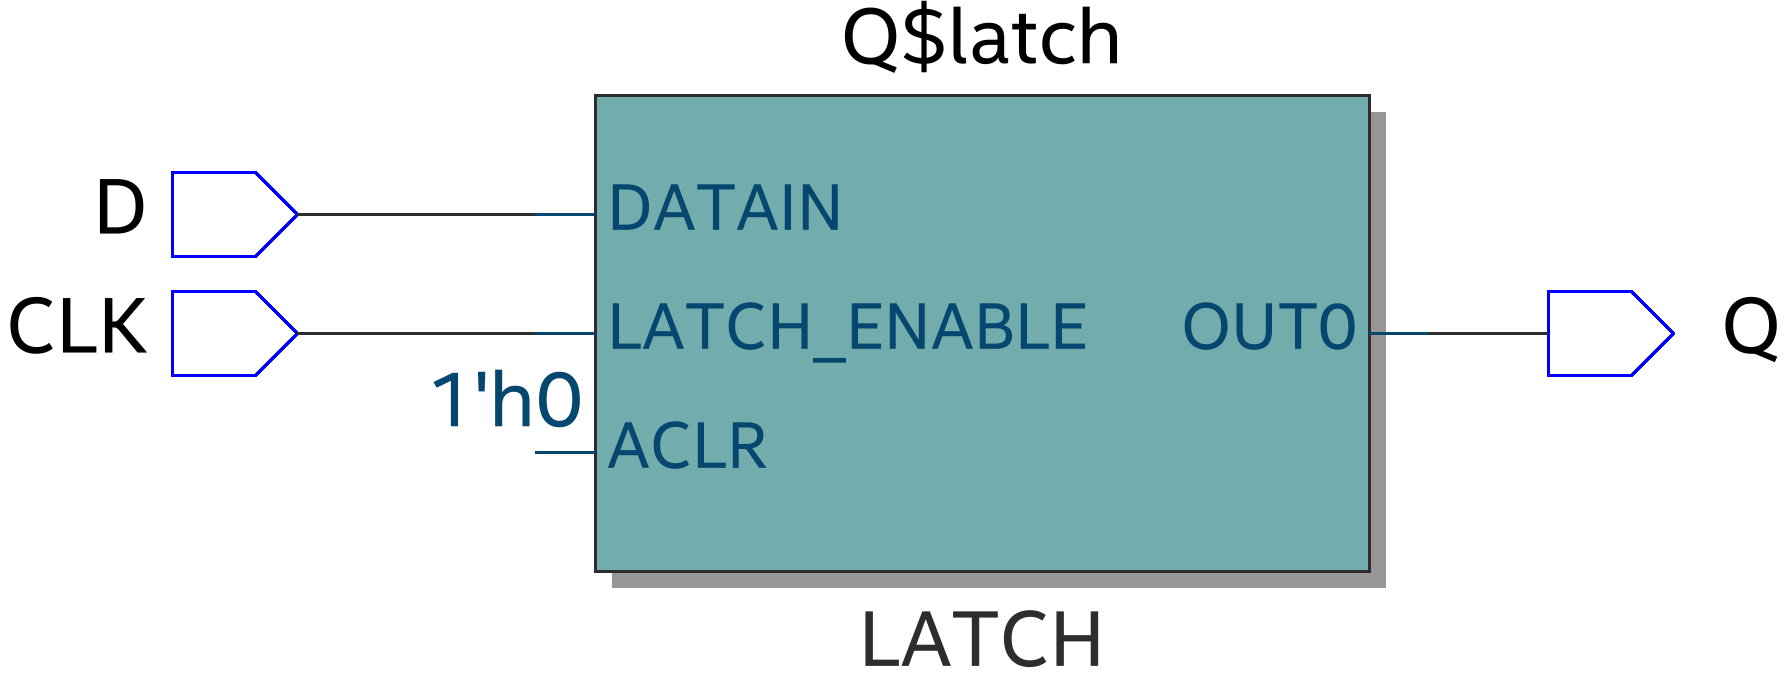
\includegraphics[scale=0.34]{L_D_RTL.png}
	\caption{Diagrama RTL del latch D, descrito por comportamiento. \label{fig:L_D_RTL}}
\end{figure}

\begin{figure}[ht]
	\centering
	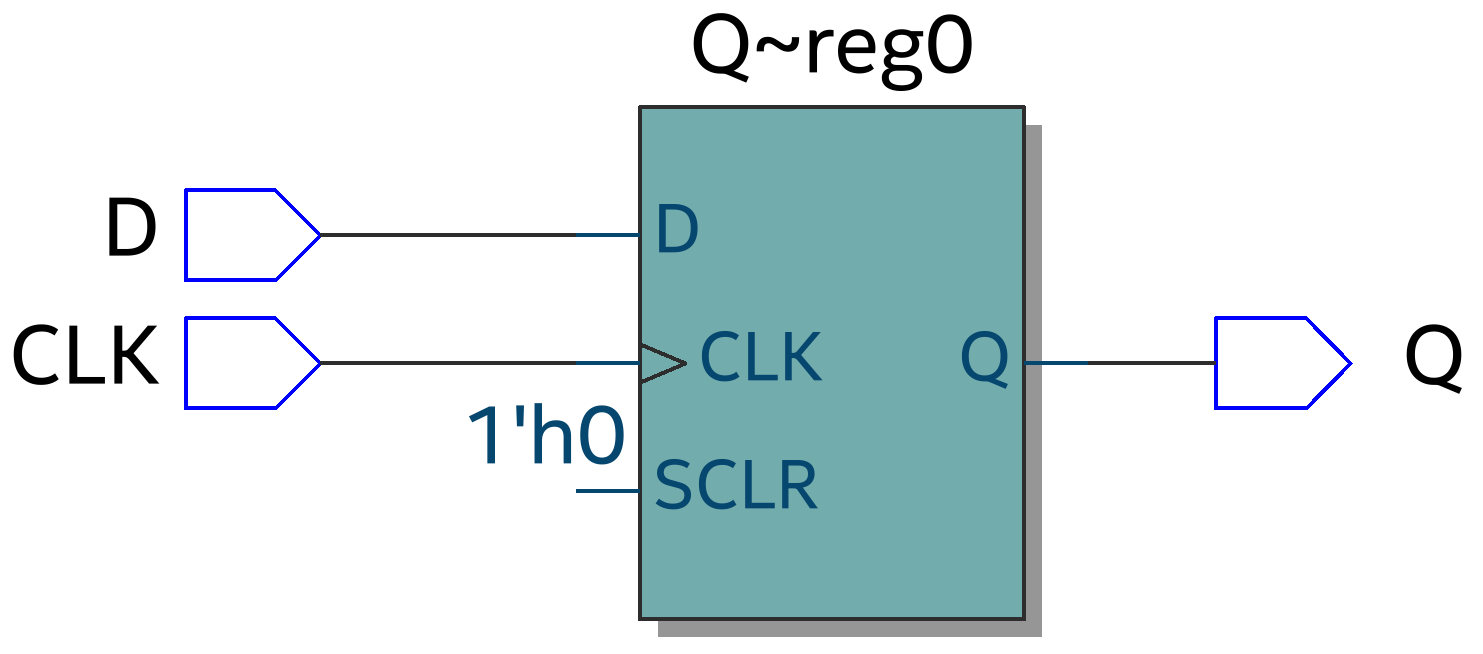
\includegraphics[scale=0.4]{FF_D_RTL.png}
	\caption{Diagrama RTL del flip-flop D, descrito por comportamiento. \label{fig:FF_D_RTL}}
\end{figure}

\begin{figure}[ht]
	\centering
	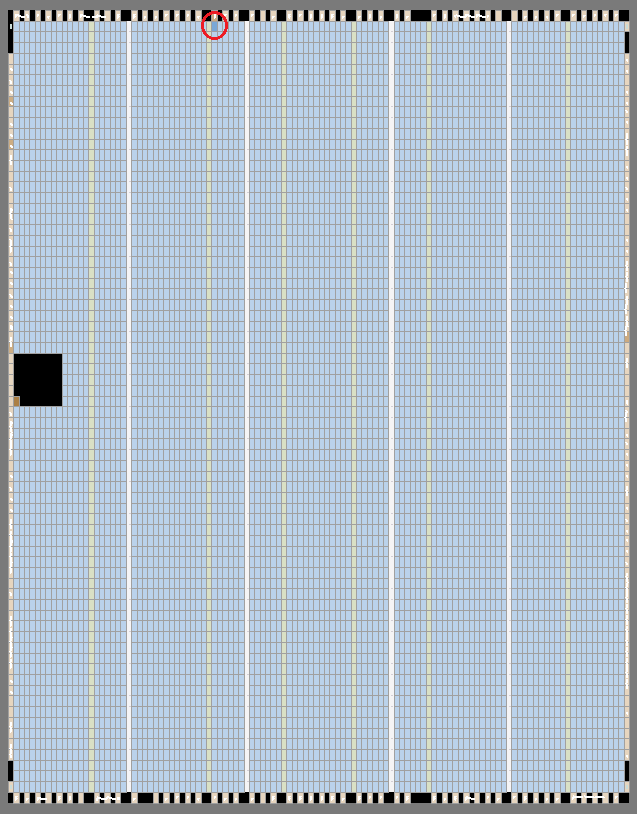
\includegraphics[scale=0.9]{L_D_CP.png}
	\caption{Latch D visto desde el \textit{Chip Planner} (círculo rojo). \label{fig:L_D_CP}}
\end{figure}

\begin{figure}[ht]
	\centering
	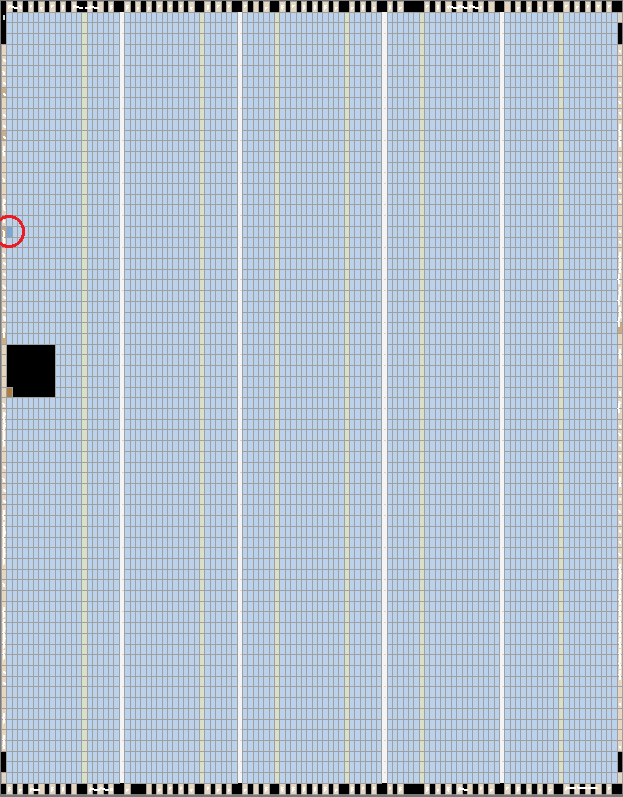
\includegraphics[scale=0.9]{FF_D_CP.png}
	\caption{Flip-Flop D visto desde el \textit{Chip Planner} (círculo rojo). \label{fig:FF_D_CP}}
\end{figure}

\begin{figure}[ht]
	\centering
	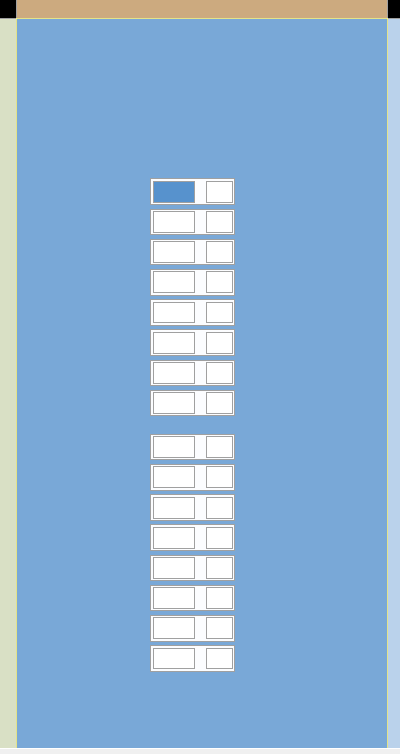
\includegraphics[scale=0.6]{L_D_CP2.png}
	\caption{Latch D visto desde el \textit{Chip Planner} (acercamiento). \label{fig:L_D_CP2}}
\end{figure}

\begin{figure}[ht]
	\centering
	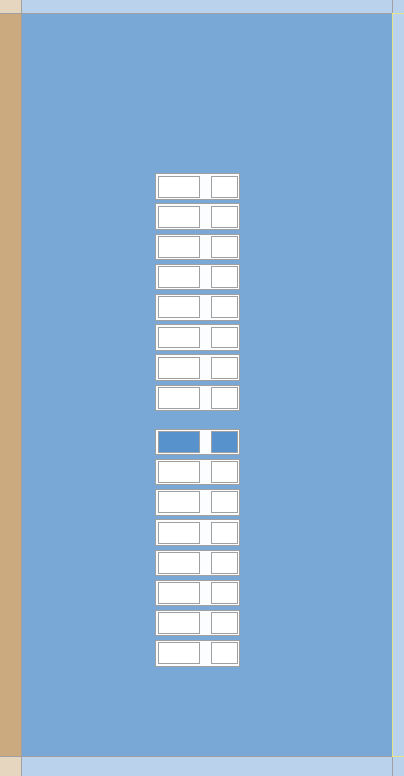
\includegraphics[scale=0.6]{FF_D_CP2.png}
	\caption{Flip-Flop D visto desde el \textit{Chip Planner} (acercamiento). \label{fig:FF_D_CP2}}
\end{figure}

\begin{figure}[ht]
	\centering
	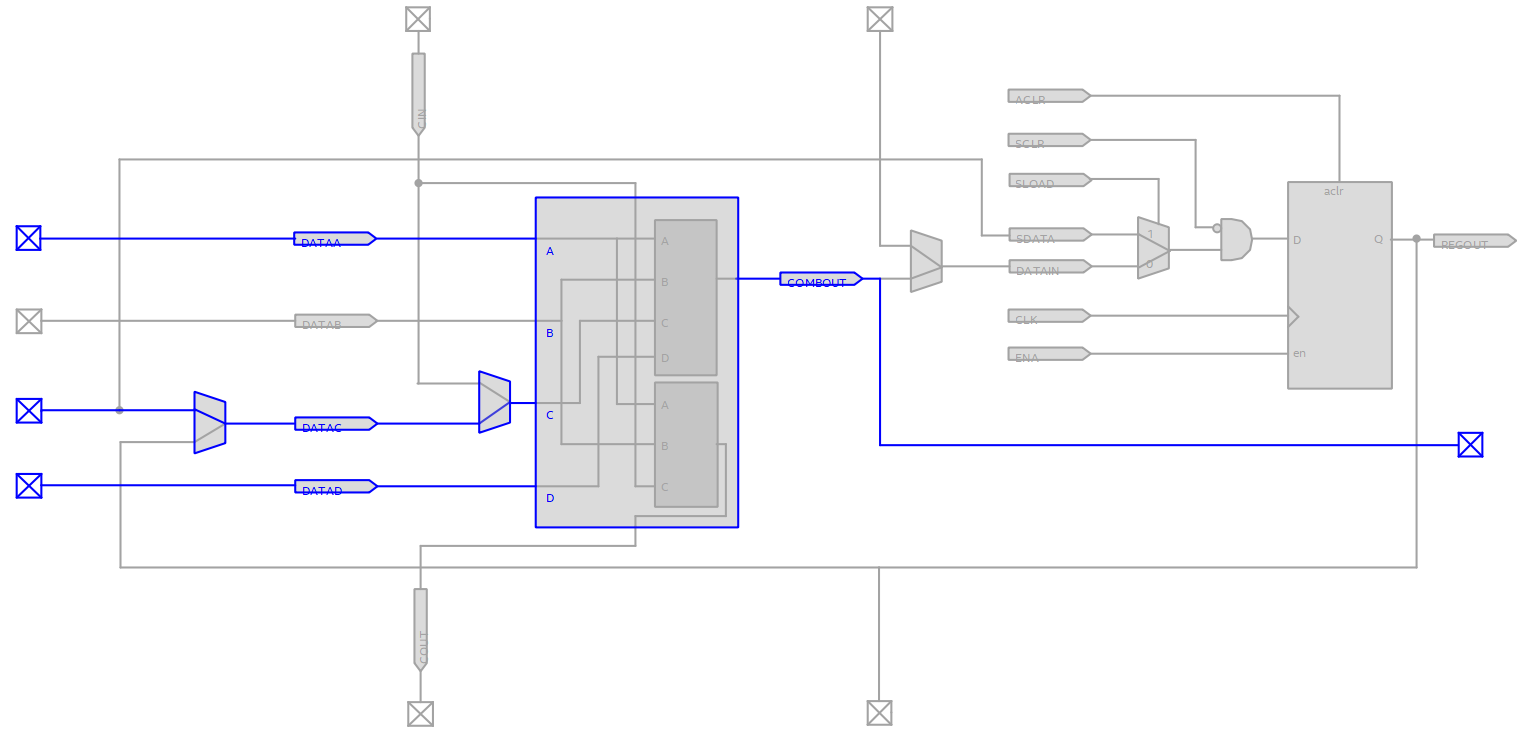
\includegraphics[scale=0.4]{L_D_CP3.png}
	\caption{Latch D visto desde el \textit{Chip Planner} (implementación en \textit{Look Up Table} del elemento lógico). \label{fig:L_D_CP3}}
\end{figure}

\begin{figure}[ht]
	\centering
	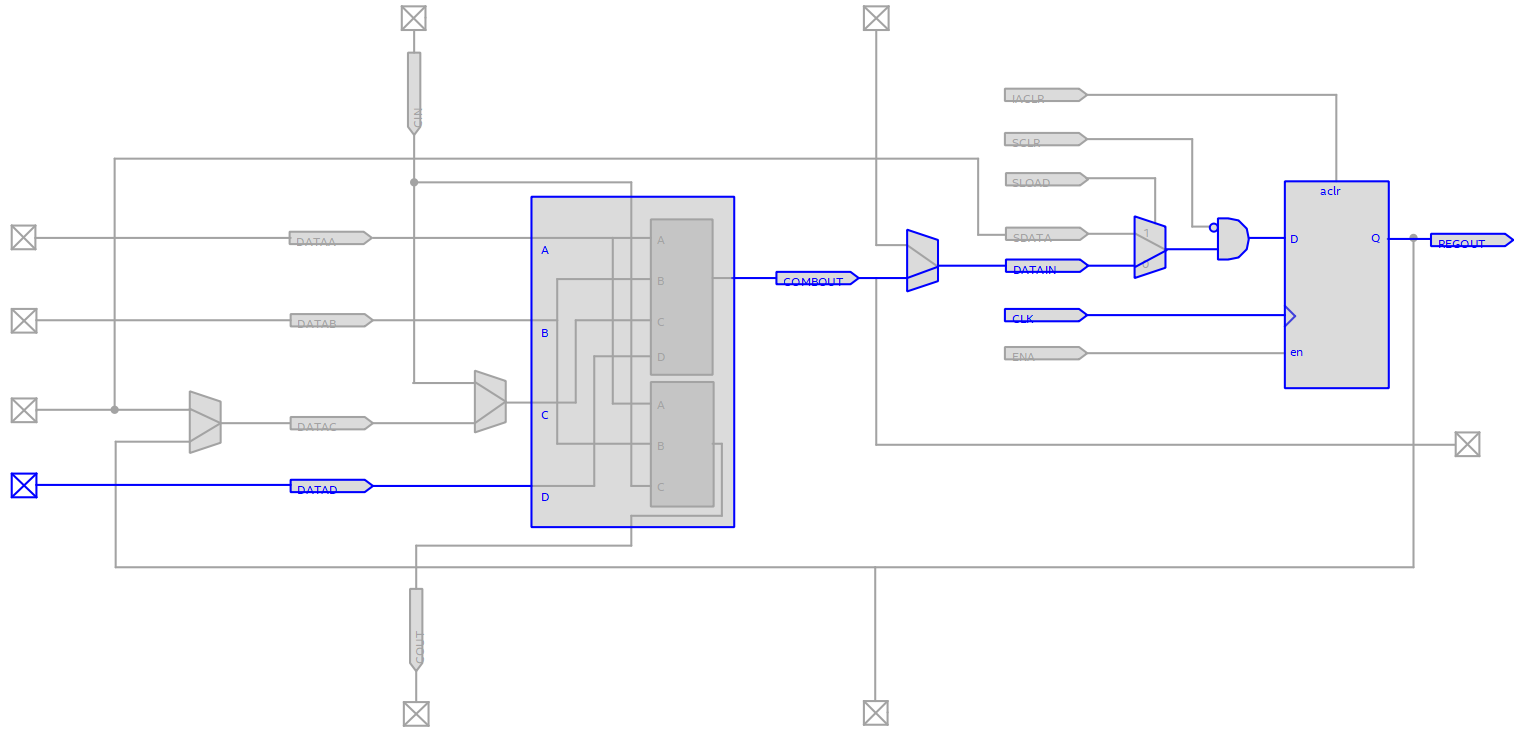
\includegraphics[scale=0.4]{FF_D_CP3.png}
	\caption{Flip-Flop D visto desde el \textit{Chip Planner} (implementación en elemento lógico). \label{fig:FF_D_CP3}}
\end{figure}

\begin{figure}[ht]
	\centering
	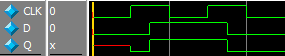
\includegraphics[scale=2]{L_D_Wave.png}
	\caption{Simulación del latch D en el visor de formas de onda de ModelSim. \label{fig:L_D_Wave}}
\end{figure}

\begin{figure}[ht]
	\centering
	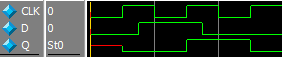
\includegraphics[scale=2]{FF_D_Wave.png}
	\caption{Simulación del flip-flop D en el visor de formas de onda de ModelSim. \label{fig:FF_D_Wave}}
\end{figure}